\chapter{Simulação}\label{simula}

\section{Execução do modelo}

Esse capítulo apresenta os resultados encontrados em cada etapa, no processo de desenvolvimento do modelo de predição de ocorrências nas principais BRs do estado de Pernambuco, para definição de melhores rotas e horários para os usuários dessas vias.

\vspace{5mm}

A figura a seguir resume as três etapas contempladas na proposição do modelo.

\begin{figure}[ht]
\centering
\caption{Etapas da modelo proposto}
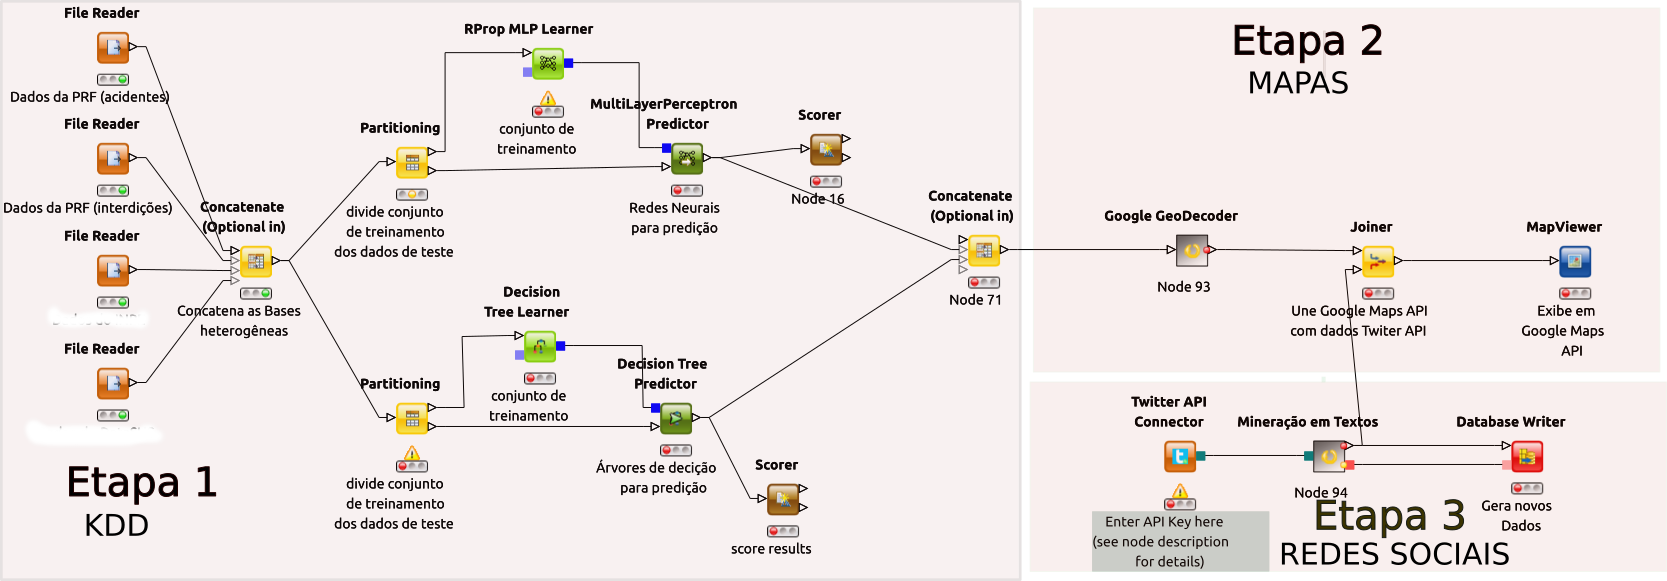
\includegraphics[width=175mm, height=75mm]{Figuras/Cronograma/metodologia.png}\\
\tiny Fonte: autor
\end{figure}

A \textbf{etapa 1} contempla a fase da coleta das bases de dados históricos, preparação dos dados, construção das variáveis do modelo preditivo, descoberta dos pontos críticos das rodovias (que serão utilizados na etapa de georreferencaimento).
  \begin{enumerate}
    \item O modelo preditivo integra as bases de dados da Polícia Rodoviária Federal -- PRF.
 
    \item Algumas dessas informações também estão disponíveis em base de dados abertas, como sugere o Portal da Transparência, nos servidores da PRF, além de outras informações complementares.
    \item A conclusão dessa etapa ocorre com a Mineração dos dados e a extração de conhecimento.
	  Os ''outputs`` dessa etapa consistem nos pontos críticos localizados nas rodovias, que permitem traçar uma rota. 
	  As localizações geográficas, indicadas pelo Km, são agrupadas formando ''clusters`` de dados exibidos em mapas vetoriais. 
	  A partir da definição dos pontos críticos foram geradas matrizes -- de mortos e de gravidade -- que serviram para localizar tais pontos no mapa e traçar rotas.
	  As principais ferramentas de I.A. utilizadas nessa etapa foram Árvores de Decisão e Redes Neurais, com a finalidade classificar e predizer os pontos críticos em cada quilômetro das rodovias.\\
\end{enumerate}
  
A \textbf{segunda} etapa contempla:
 \begin{enumerate}
 	\item Um módulo dinâmico onde são capturados ``feeds'' da rede social Twitter. 
 	     Essa técnica faz um arco cibernético mantendo o utilizador atualizado com as informações recentes. 
  \end{enumerate}

A \textbf{terceira} e última etapa consiste em um módulo com as seguintes características:
  \begin{enumerate}
    \item Representação da malha viária em mapas de bases vetoriais;
    \item Um ambiente de simulação interativa que utiliza uma plataforma baseada na API do Google Maps.
    \item Quando houver informações vindas do twitter sobre ocorrências na rodovia, deverá ser feita a geolocalização
  \end{enumerate}


\section{A construção do Modelo preditivo}

O modelo preditivo foi construído utilizando bases de dados históricos da PRF (de acidentes e de paralisações, por exemplo,  protestos) entre Janeiro de 2007 a Dezembro 2015. Cada ano correspondia a uma base de dados independentes, tendo sido integradas, formando uma base única com aproximadamente 85 mil registros. 


\subsection{Aplicação do CRISP-DM}
O CRISP-DM nesta pesquisa ajudou a guiar as escolhas nos momentos em que os resultados pareciam não fazer sentido. Todavia, por ser um processo recursivo, o retorno aos fundamentos dessa metodologia prevê que haja ajustes necessários, a fim de se atingir os objetivos da proposta.

A proposta metodológica delineada para esta pesquisa contemplou todas as fases do KDD, conforme descrito a seguir.

\subsubsection{Fases da Mineração ao KDD}

Seleção: Nesta etapa foram coletadas as informações provenientes das bases de dados da Policia Rodoviária Federal de Pernambuco entre 2007 e 2015. Segundo informações da própria PRF/PE, apenas a partir de 2007 esses dados passaram a ser armazenados eletronicamente. A PRF/PE dispõe em banco de dados relacionais alguns desses dados na Internet,
contudo no artigo “Uma análise da qualidade dos dados relativos aos boletins de ocorrências das rodovias federais para
o processo de Mineração de Dados”, COSTA, BERNARDINI, LIMA \cite{Costa2015} destacam a não padronização e não aceitação dos
dados pela comunidade internacional. EAVES, D. \cite{Eaves} sugere que os dados sejam disponibilizados na maneira como foram
coletados. 

A primeira base de dados coletada diretamente dos servidores da PRF continha relatório de acidentes e a segunda a de interdições. A partir dos dados capturados na base da PRF utilizamos como variáveis de entrada:

\begin{itemize}
 \item Condição da Pista: {Seca, Com buracos, Molhada, Em obras, Com material granulado, Oleosa, Enlameada, Com gelo, Outras}
 \item Restrição de visibilidade: {Inexistente, Veículo Estacionado, Poeira/Fumaça/neblina, Vegetação, Ofuscamento, Cartazes/faixas, Placas}
 \item Traçado da via: {Reta, Curva, Cruzamento, Defeito}
 \item Tipo de veículo: {Automóvel, Caminhonete, Motocicletas, Caminhão, Caminhão-trator, Bicicleta, Ônibus, Motoneta, Micro-ônibus, Trator de rodas, Carroça, Caminhão-Tanque, Semi-Reboque, Utilitário, Ciclomotor, Charrete, Carro-de-mão, Quadriciclo, Trator misto, Reboque, Trator de esteiras, Não informado, Não se aplica, Não identificado}
\end{itemize}

Preprocessamento: Nesta fase foram retiradas as variáveis que continham inconsistência e “missing data”, como, por exemplo, informações acerca de latitude e longitude. Cabe destacar que a base de dados, como um todo, apresentava sérias inconsistências, uma vez que, por exemplo,
um mesmo acidente, quando envolvia dois ou mais veículos,
era lançado na base duas ou mais vezes, em função da
quantidade de veículos envolvidos. Foram eliminadas variáveis
em duplicidade (i.e. as variáveis Mês, Ano que apareciam
separadamente, já haviam sido contempladas na variável Data.).

Transformação: Foram criadas as variáveis “Tipo de
paralisação”, contemplando acidentes sem mortos e com, no
máximo, dois veículos envolvidos; “Dias da semana”
(domingo, segunda-feira,....sábado); “Ajuste de horas” (i.e. 17h58, 17h59, 18h, 18h01, 18h02, arredondadas para 18h);
“Ajuste de Km” (seguiu a mesma lógica do ajuste de horas).

Mineração de dados: O algoritmo escolhido para essa fase da pesquisa
foi Árvore de Decisão, que possibilita uma interpretação
imediata e de fácil compreensão. Como ferramentas, foram
escolhidas o Knime \cite{Knime}, R \cite{R-cran} e Weka \cite{Weka}, com objetivo
de estabelecer uma comparação entre eles, cuja intenção era
produzir um classificador mais robusto. Nessa direção, a
técnica Ensamble de classificadores \cite{Bernardini} estabelece que a
combinação de um ou mais classificadores iguais, ou mais de
um classificador diferente, aumenta a precisão. 

Tanto na ferramenta Knime como Weka o algoritmo de árvore de decisão é chamado de J48,
uma vez que se trata da implementação Java do algoritmo
C4.5 no R. A biblioteca “rparty” implementa esse algoritmo.

Para escolha das variáveis de entrada foi calculada a correlação linear entre todas as variáveis. Entre as variáveis BR e
Delegacia (variável que agrega municípios) obteve-se correlação linear de 0,653. Entre Tipo de Acidente e Traçado via a
correlação foi baixa, apenas 0,14. Variáveis com correlação linear abaixo disso foram descartadas. 

Outra métrica para a escolha de variáveis de entrada foi a entropia, que é um elemento considerado importante pela literatura \cite{NorvigRussel2004}. Nesse caso, variáveis que seriam desconsideradas em virtude da baixa correlação linear, foram reconsideradas por conta da entropia.

Interpretação/Avaliação: Produção de árvores de decisão a
partir do estabelecimento de diferentes nós-raízes, definidos em
virtude da correlação linear e/ou da entropia.

\pagebreak

%++++++++++++++++++++++++++++++++++++++++++++++++++++++++++++++++++++++++++++++++++++++++++++++
\subsection{Dados encontrados antes da Mineração}

Os dados revelaram que a grande maioria dos acidentes ocorre com pista seca, sem restrição de visibilidade. 
A cor vermelha remete aos trechos BR 101 em que ocorrem mais acidentes. A cor azul diz respeito à menor frequência de acidentes.

\begin{figure}[h]
	\caption{BR 101: Hora do acidente (1) Concentração em torno da hora (2)}
	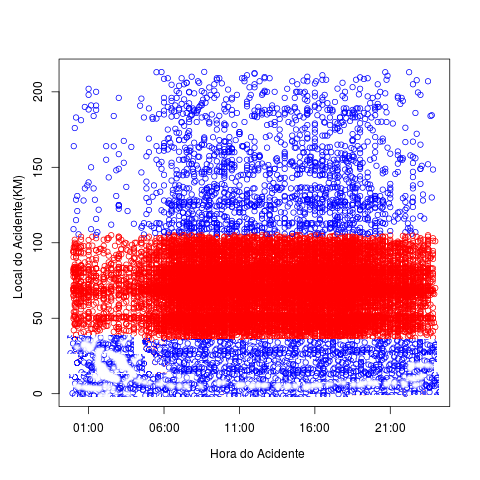
\includegraphics[width=7cm,height=7cm]{Figuras/Preprocess/br101.png}
	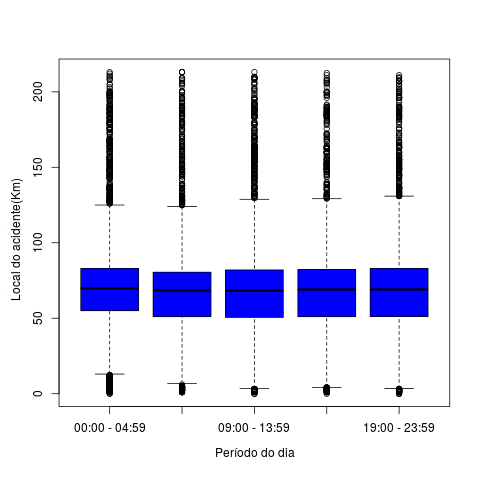
\includegraphics[width=7cm,height=7cm]{Figuras/Preprocess/br101_2.png}
	
\end{figure}

\quad \quad
\begin{figure}[h]
	\centering
	\caption{ Frequência}
	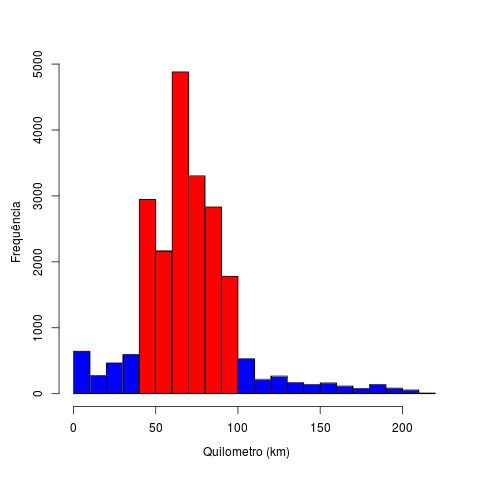
\includegraphics[width=7cm,height=7cm]{Figuras/Preprocess/br101_4.png}
\end{figure}

O gráfico 4.2(1), 4.2(2)  e 4.3 contêm dados da BR 101, uma das mais importantes para o nordeste brasileiro, uma vez que atravessa a maioria dos estados dessa região, nas localidades mais densamente povoadas. Em virtude disso, seu tráfego intenso. 
A gráfico 4.2(1) representa os acidentes que ocorreram a cada hora (abcissa) em cada Km (ordenada) nos últimos nove anos. 
O  gráfico 4.2(2) corresponde à frequência do local onde ocorreram esses acidentes. 
É possível perceber que há determinados locais na rodovia onde se concentram os acidentes. 
O terceiro gráfico, tipo ‘boxplot’, exibe a concentração das ocorrências em torno da mediana dessa localidade (Km). 
Especulou-se, a priori, que a variável “traçado da rodovia” ou que as condições climáticas poderiam ser de grande influência na ocorrência de acidentes, contudo mais adiante descobrimos outros condicionantes que influenciam mais fortemente esses acontecimentos. 
É possível perceber no gráfico 4.2(1) e no 4.3 que especialmente em determinados locais (Km) -- por exemplo na BR 101, entre os Km 40 e 100 -- os acidentes ocorrem desde as 05h da manhã até as 23h. 



\begin{figure}[h]
	\caption{BR 104: Hora do acidente (1) Concentração em torno da hora (2)}
	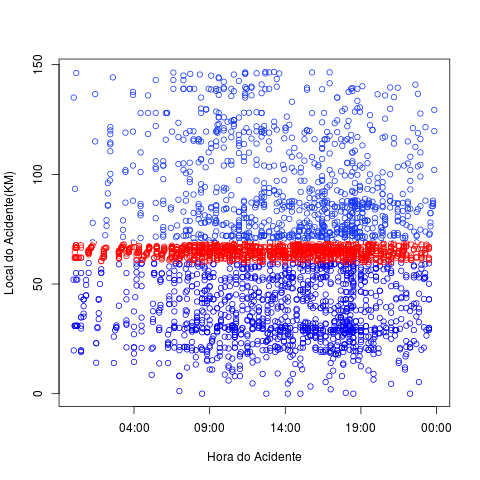
\includegraphics[width=7cm,height=7cm]{Figuras/Preprocess/br104_12.png}
	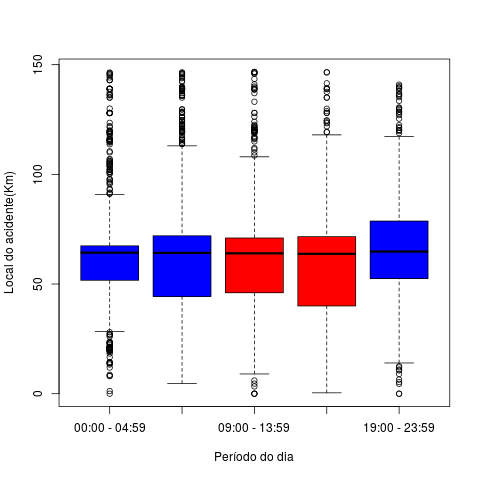
\includegraphics[width=7cm,height=7cm]{Figuras/Preprocess/br104_2.png}

\end{figure}

\quad \quad
\begin{figure}[h]
	\centering
	\caption{ Frequência}
	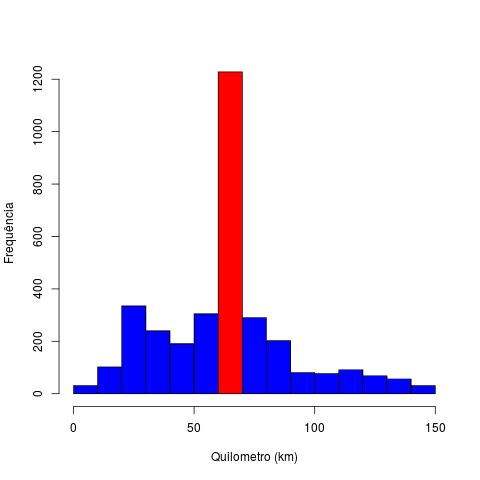
\includegraphics[width=7cm,height=7cm]{Figuras/Preprocess/br104_3.png}
\end{figure}

O gráfico 4.4(1), 4.4(2) e 4.5 apresentam dados da BR 104, que atravessa seis municípios de Pernambuco, dentre eles Caruaru, que é responsável por uma das maiores frotas de veículos do interior e por onde passam cerca de 50 mil veículos por dia. 
A gráfico 4.4(1) representa, nos últimos nove anos, os acidentes que ocorreram a cada hora (abcissa) em cada Km (ordenada).
O  gráfico 4.4(2) corresponde à frequência do local onde ocorreram esses acidentes. 
Percebe-se que em torno do Km 60 concentra-se o maior número de ocorrências. 
O terceiro gráfico (boxplot) apresenta as ocorrências em torno da mediana dessa localidade (Km). 
No gráfico 1 são identificados padrões, por exemplo no Km 60 ocorrem acidentes que se estendem das 04h às 23h. 


\pagebreak
%++++++++++++++++++++++++++++++++++++++++++++++++++++++++++++++++++++++++++++++++++++++++++++++

\begin{figure}[h]
	\caption{BR 110: Hora do acidente (1)  Concentração em torno da hora (2)}
	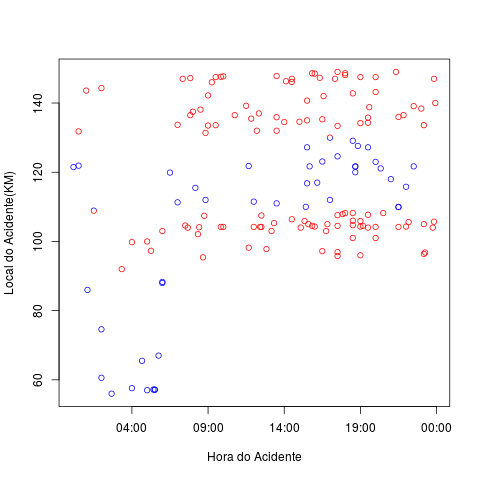
\includegraphics[width=7cm,height=7cm]{Figuras/Preprocess/br110_1.png}
	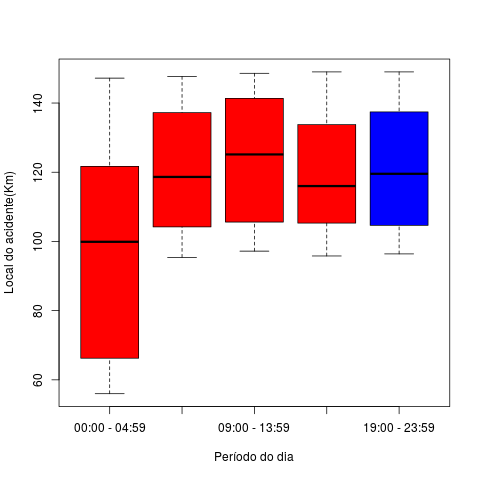
\includegraphics[width=7cm,height=7cm]{Figuras/Preprocess/br110_2.png}

\end{figure}


\quad \quad
\begin{figure}[h]
	\centering
	\caption{ Frequência}
	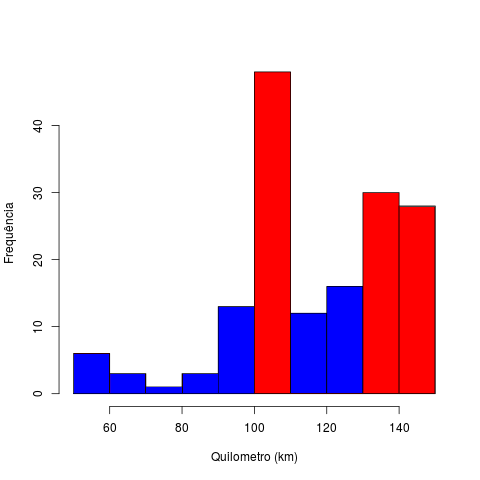
\includegraphics[width=7cm,height=7cm]{Figuras/Preprocess/br110_3.png}
\end{figure}

\pagebreak
%++++++++++++++++++++++++++++++++++++++++++++++++++++++++++++++++++++++++++++++++++++++++++++++

\begin{figure}[h]
	\caption{BR: 116 Hora do acidente (1) Concentração em torno da hora (2)}
	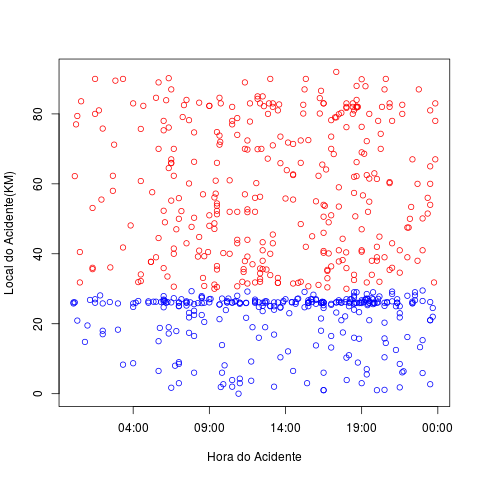
\includegraphics[width=7cm,height=7cm]{Figuras/Preprocess/br116_1.png}
	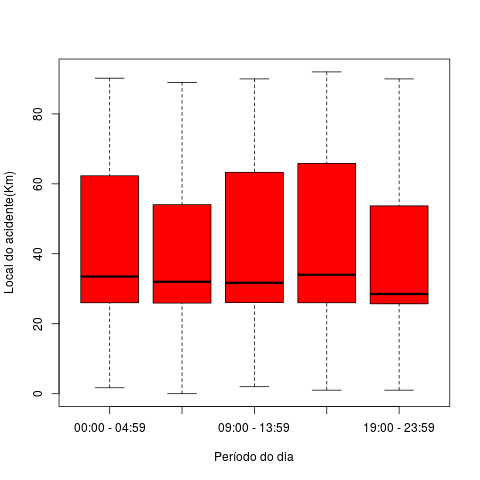
\includegraphics[width=7cm,height=7cm]{Figuras/Preprocess/br116_2.png}

\end{figure}

\quad \quad
\begin{figure}[h]
	\centering
	\caption{ Frequência}
	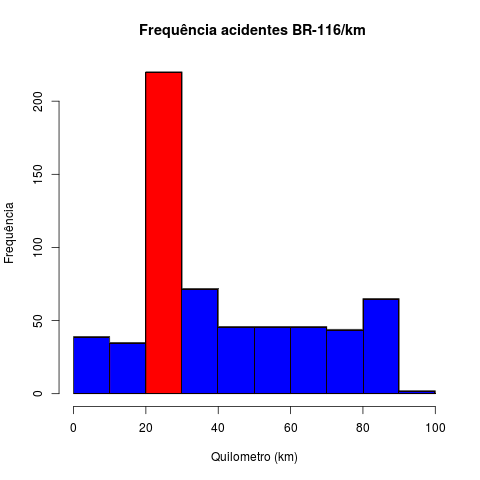
\includegraphics[width=7cm,height=7cm]{Figuras/Preprocess/br116_3.png}
\end{figure}

O gráfico 4.8(1), 4.8(2)  e 4.9 apresentam dados da BR 116, que percorre os estados do Brasil que vão desde o Rio Grande do Sul até o Ceará. O gráfico 4.8(1) mostra os acidentes que ocorreram a cada hora (abcissa) em cada Km (ordenada), também nos últimos nove anos. 
O  gráfico 4.8(2) corresponde à frequência do local onde esses acidentes aconteceram. Há determinados locais na rodovia em que a maioria dos acidentes se concentram. 
O gráfico tipo ‘boxplot’ exibe a concentração das ocorrências em torno da mediana dessa localidade (Km). 
Inicialmente acreditou-se que a variável “traçado da rodovia” ou que as condições climáticas poderiam ter grande influência na causa dos acidentes. Entretanto, mais adiante foram descobertos outros condicionantes dessas ocorrências. 
É possível perceber no gráfico 4.9, que os acidentes em torno do Km 30 ocorrem com mais frequência a partir da 04h da manhã, estendendo-se até próximo às 22h. 

\pagebreak
%++++++++++++++++++++++++++++++++++++++++++++++++++++++++++++++++++++++++++++++++++++++++++++++

\begin{figure}[h]
	\caption{BR 232: Hora do acidente (1)  Concentração em torno da hora (2)}
	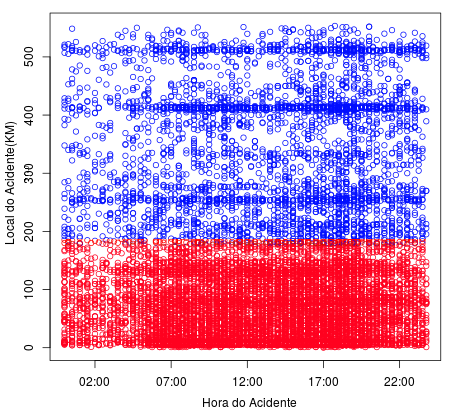
\includegraphics[width=7cm,height=7cm]{Figuras/Preprocess/br232_1.png}
	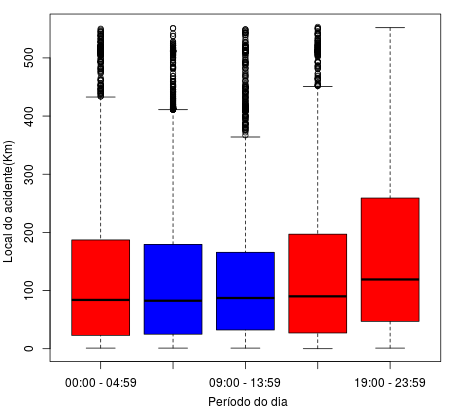
\includegraphics[width=7cm,height=7cm]{Figuras/Preprocess/br232_32.png}

\end{figure}

\quad \quad
\begin{figure}[h]
	\centering
	\caption{ Frequência}
	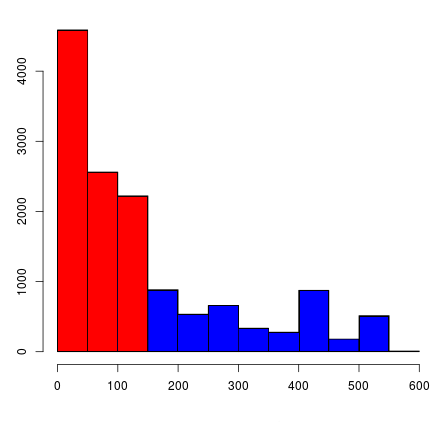
\includegraphics[width=7cm,height=7cm]{Figuras/Preprocess/br232_3.png}
\end{figure}

O gráfico 4.10(1), 4.10(2)  e 4.11 trazem dados da BR 232, cuja importância se destaca pelo fato de atravessar todo o estado de Pernambuco, de leste a oeste. O primeiro gráfico apresenta os acidentes dos últimos nove anos, em cada hora (abcissa) e Km (ordenada). O  gráfico 4.10(2) corresponde ao local onde aconteceram esses acidentes. É possível perceber no gráfico 4.11, que nessa BR há um número maior de acidentes nos Km 0, 90, 110, 260, 410 e 500, desde a 00h até as 23h. O terceiro gráfico (‘boxplot’) exibe a concentração das ocorrências em torno da mediana dessa localidade (Km). 
Especulou-se a priori que a variável “traçado da rodovia” ou que as condições climáticas eram as principais responsáveis pelo grande número de acidentes.



\pagebreak
%++++++++++++++++++++++++++++++++++++++++++++++++++++++++++++++++++++++++++++++++++++++++++++++

\begin{figure}[h]
	\caption{BR 316: Hora do acidente (1) Concentração em torno da hora (2)}
	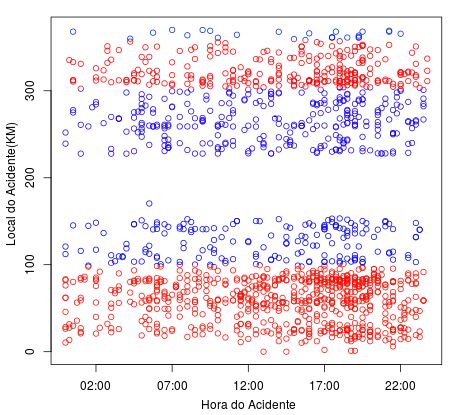
\includegraphics[width=7cm,height=7cm]{Figuras/Preprocess/br316_1.png}
	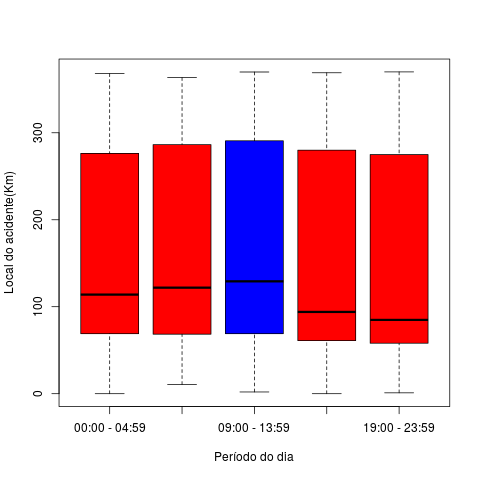
\includegraphics[width=7cm,height=7cm]{Figuras/Preprocess/br316_2.png}

\end{figure}

\quad \quad
\begin{figure}[h]
	\centering
	\caption{ Frequência}
	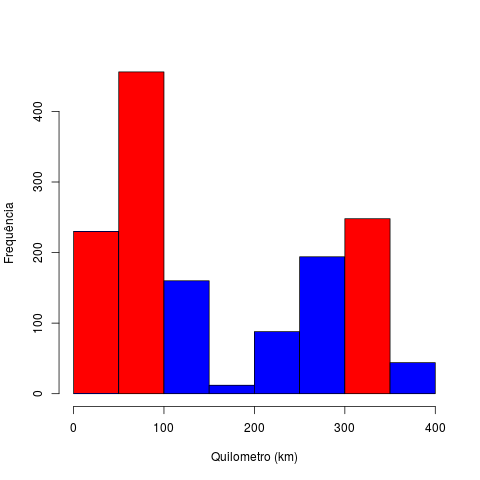
\includegraphics[width=7cm,height=7cm]{Figuras/Preprocess/br316_3.png}
\end{figure}

O gráfico 4.12(1), 4.12(2)  e 4.13 trazem dados da BR 316. Esta BR é uma das menores do Estado de Pernambuco, de oeste a leste. O primeiro gráfico apresenta uma área em branco no centro, os acidentes se concentram nas extremidades, no entorno do km 90 e 300 (da abcissa) e acontecem com maior frequência em torno das 17h00 (ordenada).

\pagebreak
%++++++++++++++++++++++++++++++++++++++++++++++++++++++++++++++++++++++++++++++++++++++++++++++

\begin{figure}[h]
	\caption{BR 407: Hora do acidente (1) Concentração em torno da hora (2)}
	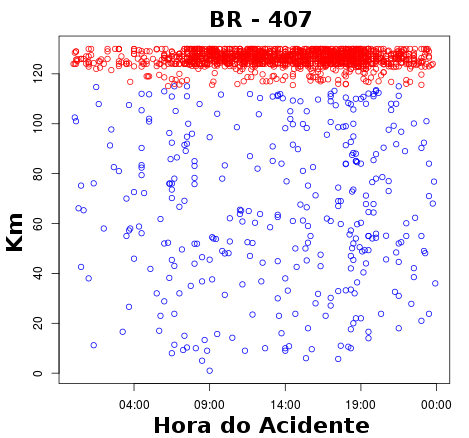
\includegraphics[width=7cm,height=7cm]{Figuras/Preprocess/br407_1.png}
	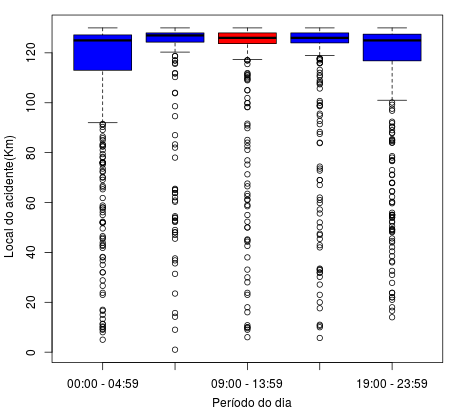
\includegraphics[width=7cm,height=7cm]{Figuras/Preprocess/br407_3.png}

\end{figure}

\quad
\begin{figure}[h]
	\centering
	\caption{ Frequência}
	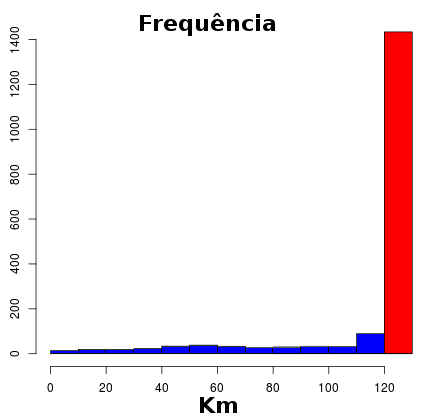
\includegraphics[width=7cm,height=7cm]{Figuras/Preprocess/br407_2.png}
\end{figure}

Na BR 407 os acidentes se concentram na altura do Km 130, representados nos gráficos 4.14 (1) e 4.14 (2).
Esta BR situa-se no extremo oeste do Estado, ligando a cidade de Afrânio a Petrolina. A peculiaridade desse trecho (km 130) é verificada na descida da ponte que atravessa o rio São Francisco.

\pagebreak
%++++++++++++++++++++++++++++++++++++++++++++++++++++++++++++++++++++++++++++++++++++++++++++++

\begin{figure}[h]
	\caption{BR 408: Hora do acidente (1) Concentração em torno da hora (2)}
	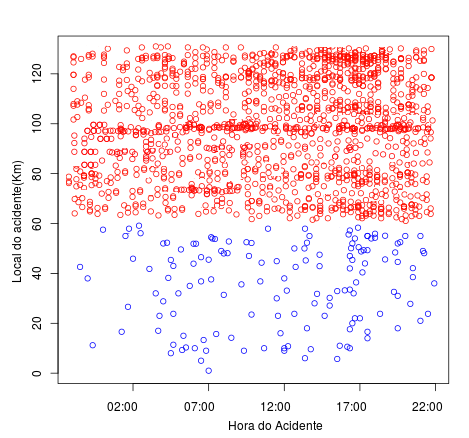
\includegraphics[width=7cm,height=7cm]{Figuras/Preprocess/br408_1.png}
	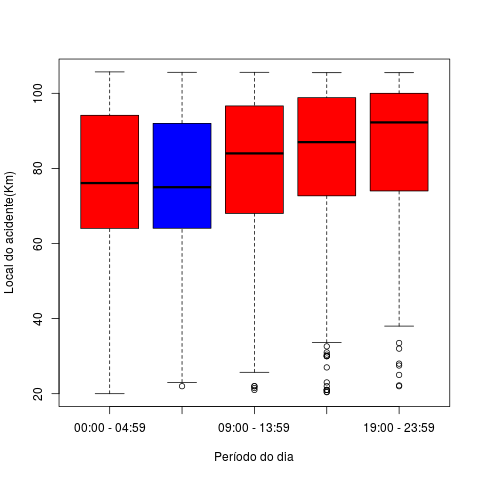
\includegraphics[width=7cm,height=7cm]{Figuras/Preprocess/br408_2.png}

\end{figure}

\quad \quad
\begin{figure}[h]
	\centering
	\caption{ Frequência}
	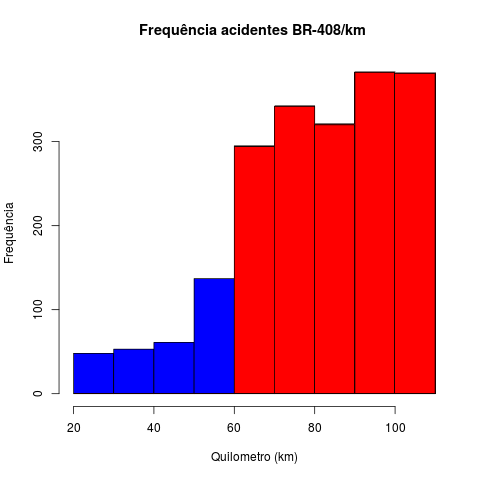
\includegraphics[width=7cm,height=7cm]{Figuras/Preprocess/br408_3.png}
\end{figure}

O gráfico 4.16 (1), 4.16 (2)  e 4.17 representam a BR 408. Em Pernambuco esta BR liga a cidade de Timbaúba a Jaboatão dos Guararapes. Esta BR tem importância a medida integra o setor industrial de autopeças no norte de Pernambuco proporcionado pela fábrica da Fiat (FCA) ligando-se ao polo industrial do sul do Estado. 
\pagebreak
%++++++++++++++++++++++++++++++++++++++++++++++++++++++++++++++++++++++++++++++++++++++++++++++

\begin{figure}[h]
	\caption{BR 423: Hora do acidente (1)  Concentração em torno da hora (2)}
	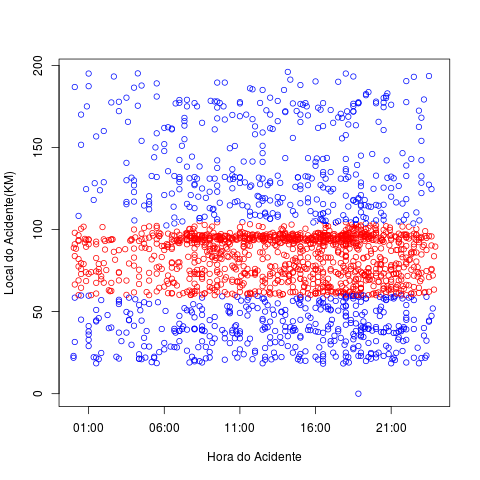
\includegraphics[width=7cm,height=7cm]{Figuras/Preprocess/br423_1.png}
	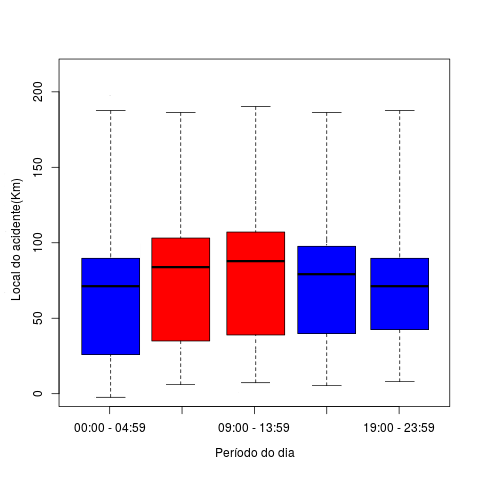
\includegraphics[width=7cm,height=7cm]{Figuras/Preprocess/br423_2.png}
	
\end{figure}

\quad \quad
\begin{figure}[h]
	\centering
	\caption{ Frequência}
	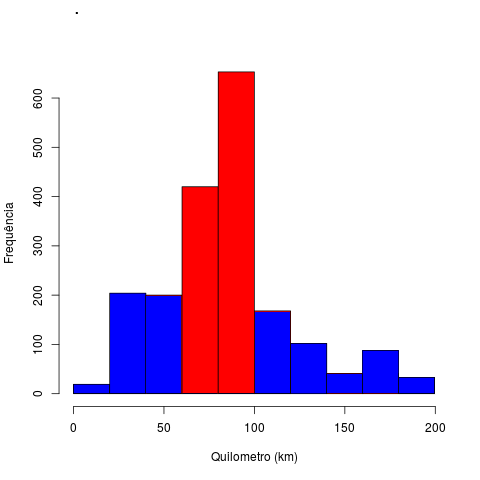
\includegraphics[width=5cm,height=6cm]{Figuras/Preprocess/br423_3.png}
\end{figure}

A BR 423 4.18 (1), 4.18 (2)  e 4.19, esta BR é a mais estratégica rodovia do Nordeste por ser o elo entre a BR 232 (a mais extensa BR do Estado de Pernambuco) à principal hidroelétrica da região; Paulo Afonso. Esta rodovia inicia-se no município de São Caetano indo até a fronteira com o estado de Alagoas no município de Itaíba, com 196,2 km é a 4ª mais extensão do Estado.
\pagebreak
%++++++++++++++++++++++++++++++++++++++++++++++++++++++++++++++++++++++++++++++++++++++++++++++

\begin{figure}[h]
	\caption{BR 424: Hora do acidente (1) Concentração em torno da hora (2)}
	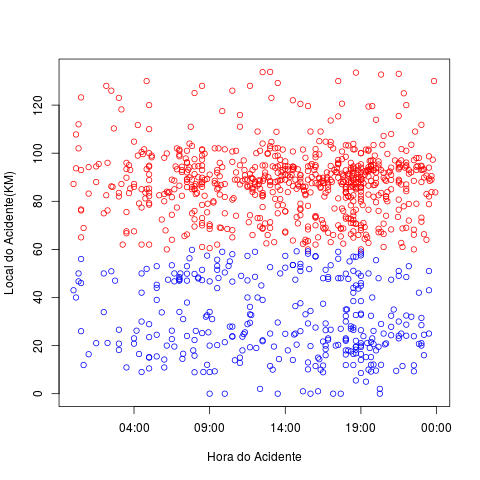
\includegraphics[width=7cm,height=7cm]{Figuras/Preprocess/br424_1.png}
	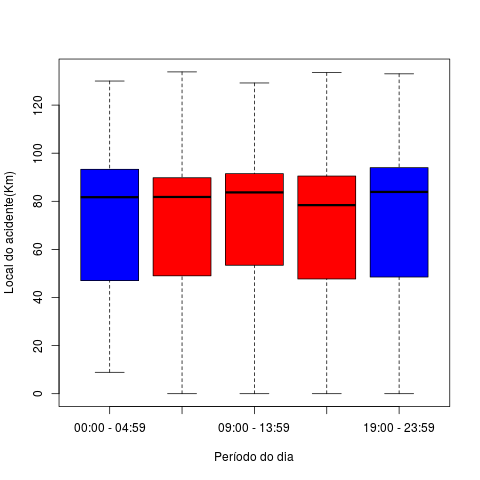
\includegraphics[width=7cm,height=7cm]{Figuras/Preprocess/br424_2.png}
	
\end{figure}

\quad \quad
\begin{figure}[h]
	\centering
	\caption{ Frequência}
	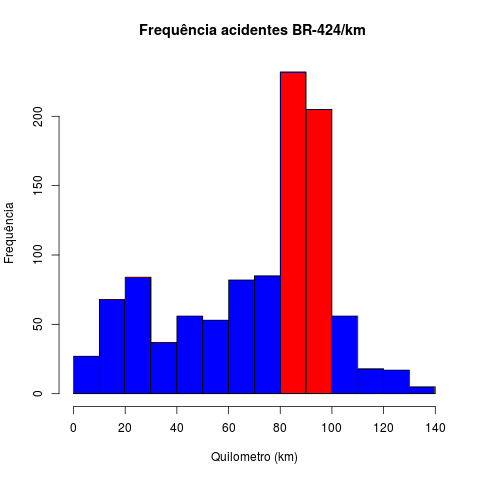
\includegraphics[width=7cm,height=7cm]{Figuras/Preprocess/br424_3.png}
\end{figure}

A rodovia BR 424 inicia em Arcoverde e termina em Correntes. Com extensão de 133,9 km tem características semelhantes à BR 423 (vide gráficos 4.20 (1 e 2) e 4.21), contudo esta rodovia tem importância secundária interligando o importante município do Agreste, Garanhuns, à BR 424.
\pagebreak
%++++++++++++++++++++++++++++++++++++++++++++++++++++++++++++++++++++++++++++++++++++++++++++++


\begin{figure}[h]
	\caption{BR 428: Hora do acidente (1) Concentração em torno da hora (2)}
	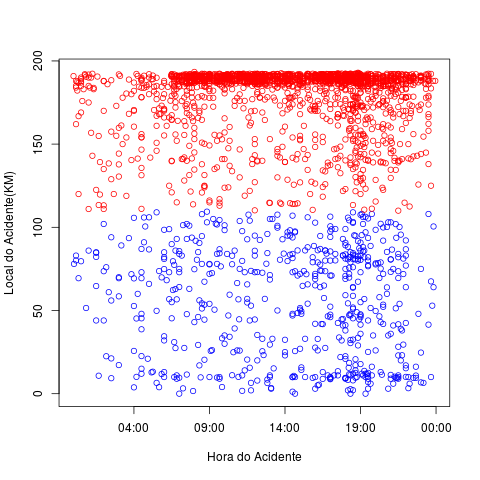
\includegraphics[width=7cm,height=7cm]{Figuras/Preprocess/br428_1.png}
	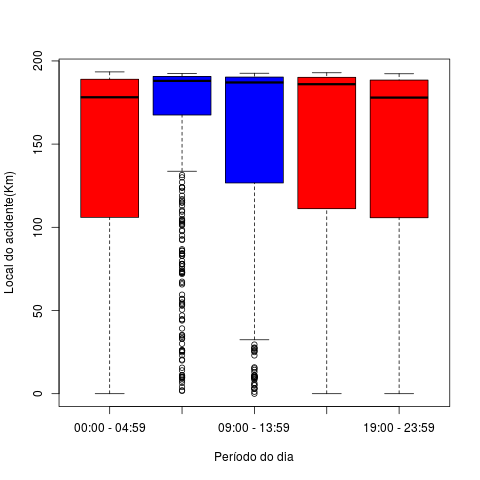
\includegraphics[width=7cm,height=7cm]{Figuras/Preprocess/br428_2.png}
	
\end{figure}

\quad \quad
\begin{figure}[h]
	\centering
	\caption{ Frequência}
	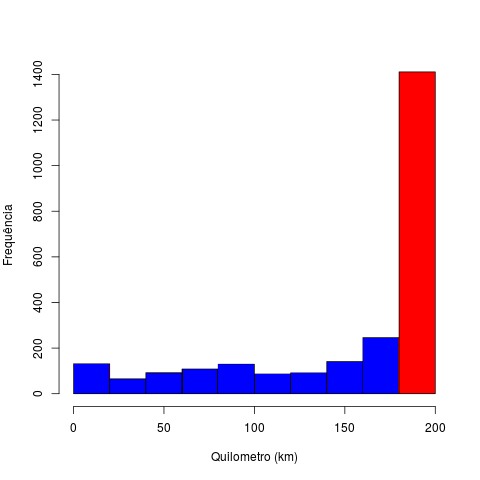
\includegraphics[width=7cm,height=7cm]{Figuras/Preprocess/br428_3.png}
\end{figure}

A BR 428 é a 11ª rodovia federal estudada nesta pesquisa, ela conecta os municípios de Belém do São Francisco ao município de Petrolina, o maior do Sertão pernambucano. Esta rodovia contorna o Rio São Francisco pela margem norte. Nesta rodovia o ponto crítico situa-se no entorno do km 180 sendo que, cerca das 19h00 o horário que ocorrem o maior número de acidentes (vide gfáfico 4.22).  
\pagebreak
%++++++++++++++++++++++++++++++++++++++++++++++++++++++++++++++++++++++++++++++++++++++++++++++

\begin{figure}[ht]
\begin{center}
\caption{Tipo de Veículo X Num. Acidentes}
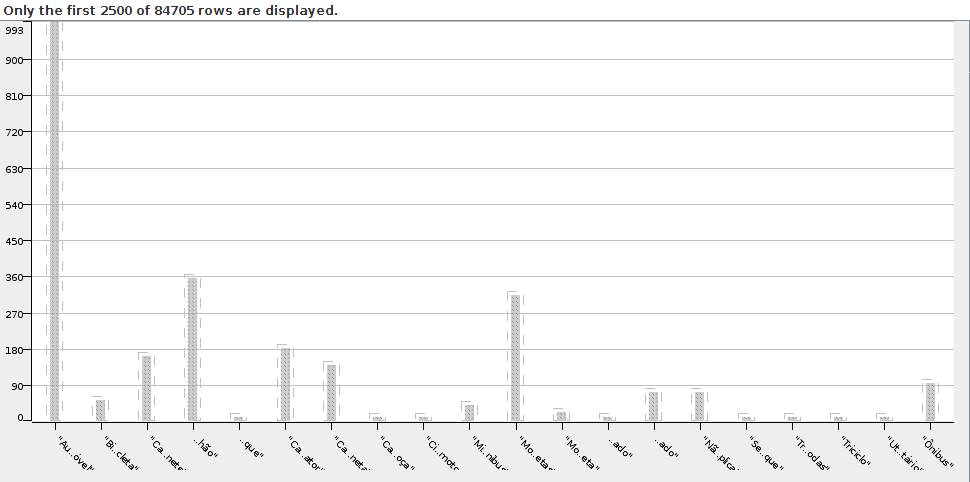
\includegraphics[width=150mm, height=90mm]{Figuras/Preprocess/TipoVeiculoXNumAciden.png}\\
\tiny Fonte: o Autor
\end{center}
\end{figure}

O número elevado de acidentes que tem por causa o automóvel de passeio que trafega por via retilínea, provavelmente condutores comuns, não profissionalizados.
O Caminhão é o segundo veículo que mais se envolve em acidentes, seguido das motonetas (motocicletas com portência limnitada). 

\pagebreak

\begin{figure}[ht]
\begin{center}
\caption{Traçado da via X Num. Acidentes}
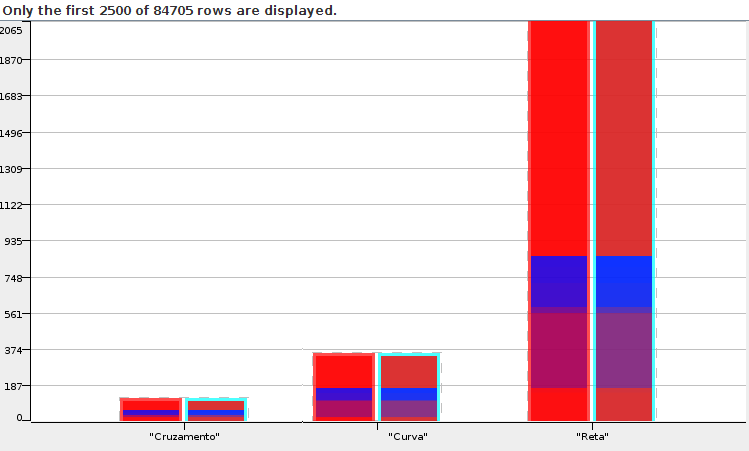
\includegraphics[width=150mm, height=50mm]{Figuras/Preprocess/TracadoViaNumAcident.png}\\
\tiny Fonte: o Autor
\end{center}
\end{figure}


Os dados do gráfico 4.25 revelam que o tipo de traçado da via (em linha reta) aparenta não influenciar a causa do elevado número de acidentes, pois a maioria dos acidentes ocorre em pista retilínea sugerindo assim que o condutor é o principal responsável pelo maior número de ocorrências nas BRs. Isso direciona essa pesquisa para analisar e antever o comportamento do condutor, perante às condições externa, além das condições da rodovia.

\pagebreak



\subsection{Dados encontrados após a Mineração}

Os resultados dos classificadores serão demonstrados a
seguir.

As variáveis “Tipo de Acidente”, “Gravidade” e
“BRajustada” foram escolhidas pelas características de ganho
de informação, dado pelo cálculo da entropia. A variável “BRajustada”
significa que essa variável foi transformada de dado numérico para categórico. A literatura \cite{NorvigRussel2004} aconselha que os nós da raiz dos classificadores, em especial Árvores de Decisão, sejam aqueles que apresentam maior
entropia, como a variável “Tipo de Acidente”.  
A seguir apresenta-se a métrica para avaliar um classificador, também conhecida como acurácia.

\begin{itemize}
	\item TP: True Positive;
	\item FP: False Positive;
	\item Prec.: Precison = TP/(TP +FP);
	\item Recall = TP/ (TP + FN);
	\item F-Me: F-measure ou f-score = 2 * Precison * Recall / (Precision + Recall);
	\item AUC: Area Under Curve (Roc);
\end{itemize}
    
\subsection{Métrica dos classificadores}

\begin{enumerate}
	\item[(i)] Variável: Tipo de Acidente (Entropia: 3.0686)
		\begin{table}[!ht]
			\centering
			%\caption{Volume de dados no mundo}
			\vspace{1mm}
			\begin{tabular}{l|c|c}
				\hline
				\textbf{Descrição} & \textbf{Valores} & \textbf{Percentual} \\
				\hline
				Instâncias Corretamente Classificadas & 7987 & 47.6324\% \\
				Instâncias Incorretamente Classificadas & 8781 & 52.3676\% \\
				Erro médio absoluto & 0.0786 & ---  \\
				Erro médio quadratico & 0.2083 & --- \\
			\end{tabular}
			\\
			\tiny Fonte: o Autor
		\end{table}
		
		\pagebreak
		
		\begin{table}[!ht]
			\centering
			\caption{Detalhe da acurácia para classe Tipo Acidente}
			\vspace{1mm}
			\begin{tabular}{l|c|c|c|c|c|l}
				\hline
				\textbf{TP} & \textbf{FP} & \textbf{Prec.} & \textbf{Recall} & \textbf{F-Me.} & \textbf{AUC} & \textbf{Classe} \\
				\hline
				0.337 & 0.059 & 0.372 & 0.337 & 0.354 & 0.738 & Colisão transversal \\
				0.026 & 0.012 & 0.066 & 0.026 & 0.038 & 0.684 & Colisão com objeto fixo \\
				0.925 &	0.003 &	0.920 & 0.925 & 0.923 & 0.980 & Atropelamento de pessoa \\
				0.463 &	0.157 &	0.448 &	0.463 &	0.455 &	0.731 &	Colisão lateral \\
				0.682 &	0.259 & 0.545 & 0.682 & 0.606 & 0.773 & Colisão traseira \\
				0.485 & 0.024 & 0.409 & 0.485 & 0.443 & 0.893 & Queda de Moto/bicicleta \\
				0.322 & 0.002 & 0.528 & 0.322 & 0.400 & 0.744 & Colisão com bicicleta \\
				0.122 & 0.026 & 0.229 & 0.122 & 0.159 & 0.786 & Capotamento \\
				0.890 & 0.014 & 0.655 & 0.890 & 0.755 & 0.954 & Atropelamento de animal \\
				0.048 & 0.007 & 0.243 & 0.048 & 0.081 & 0.729 & Colisão frontal \\
				0.440 & 0.089 & 0.366 & 0.440 & 0.399 & 0.792 & Saída de Pista \\
				0.000 & 0.000 & 0.000 & 0.000 & 0.000 & 0.658 & Colisão c/ objeto móvel\\
				0.096 & 0.006 & 0.292 & 0.096 & 0.144 & 0.774 & Tombamento \\
				0.000 & 0.000 & 0.000 & 0.000 & 0.000 & 0.616 & Derramamento de Carga \\
				0.041 & 0.000 & 0.400 & 0.041 & 0.074 & 0.627 & Danos Eventuais \\
				0.000 & 0.000 & 0.000 & 0.000 & 0.000 & 0.733 & Incêndio \\	
			\end{tabular}
			\\
			\tiny Fonte: o Autor
		\end{table}
		
		\begin{table}[!ht]
			\centering
			\caption{Matriz de confusão para a variável Tipo de acidente}
			\vspace{1mm}
			\begin{tabular}{l|c|c|c|c|c|c|c|l}
				\hline
				\textbf{a} & \textbf{b} & \textbf{c} & \textbf{d} & \textbf{e} & \textbf{f} & \textbf{g} & \textbf{h} & \textbf{Classificadores}\\
				\hline
				527 & 7 & 2 & 385 & 483 & 46 & 2 & 24 & Colisão transversal \\
				16 & 14 & 0 & 69 & 154 & 15 & 0 & 47 & Colisão com objeto fixo \\
				8 & 0 & 483 & 16 & 14 & 0 & 0 & 0 & Atropelamento de pessoa \\
				336 & 30 & 8 & 1674 & 1217 & 102 & 8 & 48 & Colisão lateral \\
				250 & 51 & 9 & 835 & 3573 & 105 & 11 & 59 & Colisão traseira \\
				44 & 4 & 1 & 74 & 120 & 266 & 2 & 0 & Queda de Moto/bicicleta \\
				8 & 0 & 0 & 22 & 38 & 3 & 38 & 1 & Colisão com bicicleta \\
				28 & 34 & 5 & 85 & 236 & 1 & 2 & 120 & Capotamento \\
				-- & -- & -- & -- & -- & -- & -- & -- & -- \\	
			\end{tabular}
			\\
			\tiny Fonte: o Autor
		\end{table}
		
		Os valores restantes foram omitidos por não representarem uma amostra
		adequada, pois a acurácia foi consideravelmente baixa, por exemplo o classificado não acerta na maioria das vezes qual a classe deve ser escolhida para todas os atributos. As variáveis de classe são as mesmas da tabela
		anterior. \\
					
%	\pagebreak	
	\item[(ii)] Variável: Gravidade (Entropia: 0,9997)
	\begin{table}[!ht]
		\centering
		%\caption{Volume de dados no mundo}
		\vspace{1mm}
		\begin{tabular}{l|c|c}
			\hline
			\textbf{Descrição} & \textbf{Valores} & \textbf{Percentual} \\
			\hline
			Instâncias Corretamente Classificadas & 12110 & 72.2209\% \\
			Instâncias Incorretamente Classificadas & 4658 & 27.7791\% \\
			Erro médio absoluto & 0.3816 & ---  \\
			Erro médio quadratico & 0.4368 & --- \\
		\end{tabular}
		\\
		\tiny Fonte: o Autor
	\end{table}
	
\pagebreak	
	
	\begin{table}[!ht]
		\centering
		\caption{Detalhe da acurácia para classe Gravidade}
		\vspace{1mm}
		\begin{tabular}{l|c|c|c|c|c|l}
			\hline
			\textbf{TP} & \textbf{FP} & \textbf{Prec.} & \textbf{Recall} & \textbf{F-Me.} & \textbf{AUC} & \textbf{Classe} \\
			\hline
			0.907 & 0.608 & 0.727 & 0.907 & 0.807 & 0.721 & S \\
			0.392 & 0.093 & 0.703 & 0.392 & 0.504 & 0.721 & N \\
				
		\end{tabular}
		\\
		\tiny Fonte: o Autor
	\end{table}
	
	\begin{table}[!ht]
		\centering
		\caption{Matriz de confusão para a variável Gravidade}
		\vspace{1mm}
		\begin{tabular}{l|c|l}
			\hline
			\textbf{a} & \textbf{b} & \textbf{Classificadores}\\
			\hline
			9747 & 996 & a = S \\
			3662 & 2363 & b = N \\
		\end{tabular}
		\\
		\tiny Fonte: o Autor
	\end{table}
	
	
	\item[(iii)] Variável: BRajustada (Entropia: 2,4128)
	\begin{table}[!ht]
		\centering
		%\caption{Volume de dados no mundo}
		\vspace{1mm}
		\begin{tabular}{l|c|c}
			\hline
			\textbf{Descrição} & \textbf{Valores} & \textbf{Percentual} \\
			\hline
			Instâncias Corretamente Classificadas & 13507 & 80.5522\% \\
			Instâncias Incorretamente Classificadas & 3261 & 19.4478\% \\
			Erro médio absoluto & 0.0469 & ---  \\
			Erro médio quadratico & 0.1656 & --- \\
		\end{tabular}
		\\
		\tiny Fonte: o Autor
	\end{table}
	
	\begin{table}[!ht]
		\centering
		\caption{Detalhe da acurácia para classe BR}
		\vspace{1mm}
		\begin{tabular}{l|c|c|c|c|c|l}
			\hline
			\textbf{TP} & \textbf{FP} & \textbf{Prec.} & \textbf{Recall} & \textbf{F-Me.} & \textbf{AUC} & \textbf{Classe} \\
			\hline
			0.902 & 0.178 & 0.812 & 0.902 & 0.854 & 0.917 & BR101 \\
			0.873 & 0.003 & 0.957 & 0.873 & 0.913 & 0.992 & BR104 \\
			0.213 & 0.001 & 0.357 & 0.213 & 0.267 & 0.816 & BR110 \\
			0.457 & 0.003 & 0.669 & 0.457 & 0.543 & 0.961 & BR116 \\
			0.760 & 0.068 & 0.787 & 0.760 & 0.774 & 0.919 & BR232 \\
			0.893 & 0.006 & 0.800 & 0.893 & 0.844 & 0.985 & BR316 \\
			0.951 & 0.007 & 0.857 & 0.951 & 0.901 & 0.995 & BR428 \\
			0.761 & 0.012 & 0.693 & 0.761 & 0.725 & 0.974 & BR423 \\
			0.461 &	0.006 &	0.599 & 0.461 &	0.521 & 0.957 & BR424 \\
			0.814 & 0.001 & 0.961 & 0.814 & 0.881 & 0.999 & BR407 \\
			0.158 & 0.010 & 0.460 & 0.158 & 0.235 & 0.781 & BR408 \\
		\end{tabular}
		\\
		\tiny Fonte: o Autor
	\end{table}
	
	\begin{table}[!ht]
		\centering
		\caption{Matriz de confusão para a variável BRajustada}
		\vspace{1mm}
		\begin{tabular}{l|c|c|c|c|c|c|c|l}
			\hline
			\textbf{a} & \textbf{b} & \textbf{c} & \textbf{d} & \textbf{e} & \textbf{f} & \textbf{g} & \textbf{h} & \textbf{Classificadores}\\
			\hline
			6960 & 0 & 0 & 625 & 0 & 0 & 0 & 0 & BR101 \\
			0 & 1071 & 0 & 156 & 0 & 0 & 0 & 0  & BR104 \\
			0 & 0 & 0 & 625 & 0 & 0 & 26 & 11  & BR110 \\
			0 & 0 & 85 & 0 & 90 & 11 & 0 & 0  & BR116 \\
			970 & 9 & 0 & 3185 & 1 & 0 & 1 & 0  & BR232 \\
			0 & 0 & 27 & 11 & 377 & 7 & 0 & 0  & BR316 \\
			0 & 0 & 0 & 0 & 0 & 95 & 0 & 0  & BR407 \\
			643 & 0 & 0 & 66 & 0 & 0 & 0 & 0  & BR408 \\
			0 & 39 & 0 & 0 & 0 & 0 & 449 & 92  & BR423 \\
			0 & 0 & 0 & 625 & 0 & 0 & 172 & 154  & BR424 \\
			0 & 0 & 15 & 0 & 3 & 675 & 0 & 0  & BR428 \\			
		\end{tabular}
		\\
		\tiny Fonte: o Autor
	\end{table}	

\end{enumerate}

A área sob a curva ROC, AUC (Area Under Curve) mede a
relação de verdadeiros positivos contra os falsos positivos.
Quanto maior a área da curva tanto melhor será o
classificador. Portanto, um número de verdadeiros positivos
acima de 80\% e o número de falsos positivos próximo a 0\%
traduzem uma área da curva ROC (AUC) que dá maior confiabilidade
aos testes.

A variável “BRajustada” não teve o maior coeficiente de
entropia encontrado, contudo esta variável apresentou
índices de classificação das instâncias corretas acima dos 80\% e
o menor índice de classificação incorreta dentre os três
classificadores utilizados. Esta variável foi a escolhida para
encabeçar os algoritmos para os resultados encontrados. 

\pagebreak

A árvore construída pelo Knime para a mesma variável “Causa do Acidente” => velocidade incompatível é apresentada na
próxima figura.

\begin{figure}[!ht]
\centering
\caption{Árvore de Decisão gerada pelo Knime}
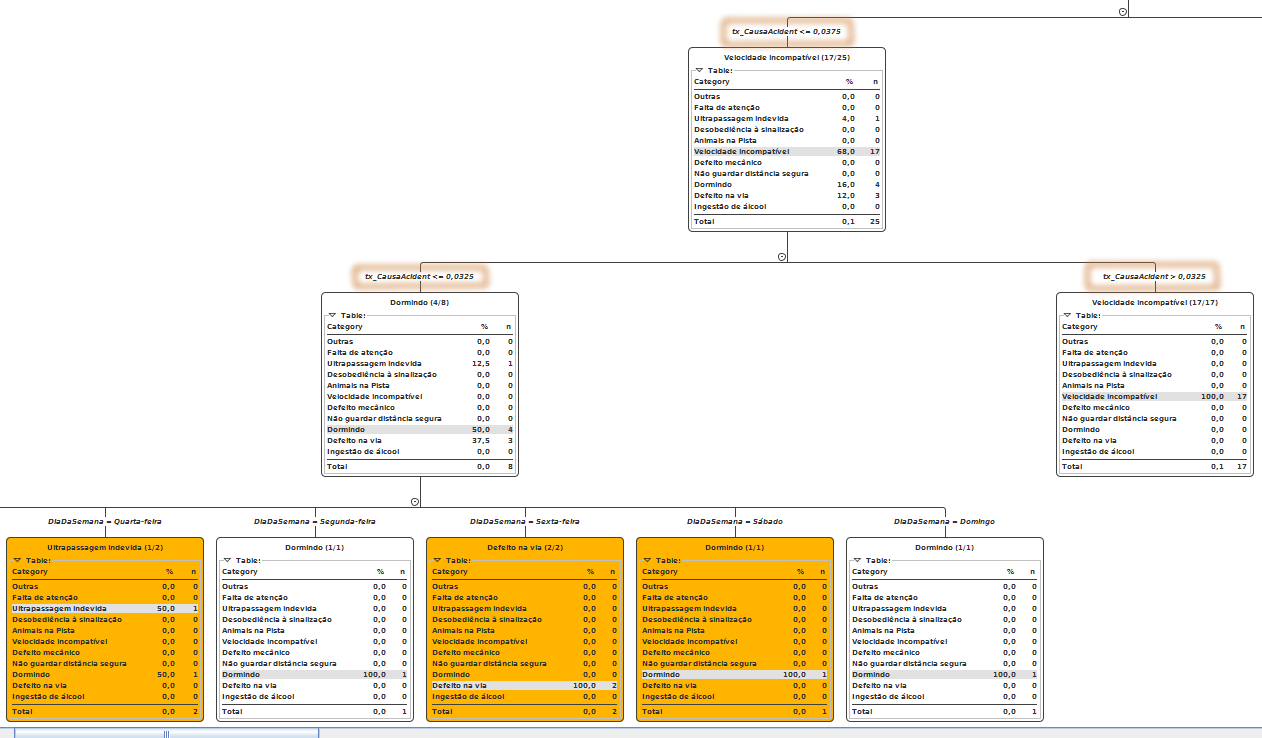
\includegraphics[width=150mm, height=145mm]{Figuras/Metodologia/arvoreKnime.png}
\label{fig:arvoreKnime}
\end{figure}

\pagebreak


Também para exemplificar, o nó folha classificou como causas dos acidentes: nas
quartas-feiras “ultrapassagem indevida”; nas sextas-feiras
“defeito na via”; e no sábado, “dormindo ao volante”.
Contudo, os melhores resultados, de acordo com mais alta
precisão, segundo a métrica dos classificadores, foi a variável
“BRajustada”, com curva ROC acima dos 90% em quase todas
as classes. O classificador Naïve Bayes obteve um
desempenho semelhante com essa
variável. Somente na BR 408 e BR 110 ficou abaixo, o que
confirma os valores encontrados pelo Weka.
Os valores das regras encontradas pelo algoritmo para a
variável “Delegacia” foram:

(a) “Delegacia” [1101(Região Metropolitana)], [BR 101],
[KM: 4], [Traçado da via: Reta], [Gravidade = S (acidente com
mortes) = 
[Causa Acidente: Falta atenção]
[Causa Acidente: Velocidade incompatível]
[Causa Acidente: Ultrapassagem indevida]
[Causa Acidente: Defeito mecânico]
[Causa Acidente: Não guardar distância]
[Causa Acidente: Dormindo]
[Causa Acidente: Ingestão de álcool]

(b) “Delegacia” [1101(Região Metropolitana)], [BR 232],
[KM: 17], [Condição pista: Seca], [Tipo Auto: automóvel]=
[Causa Acidente: Velocidade incompatível]
[Causa Acidente: Ultrapassagem indevida]
[Causa Acidente: Desobediência à sinalização]
[Causa Acidente: Não guardar distância]
[Causa Acidente: Dormindo]
[Causa Acidente: Ingestão de álcool]

Essa variedade de causas explica que o condutor dessa
região não respeita a sinalização, os limites de velocidade, dentre outros regras de trânsito. Pode-se dizer que é um condutor
indisciplinado, pois todas as causas de acidentes elencadas foram encontrados.
Caso se considere um raio de 50 Km no entorno da capital Recife, acredita-se que os motoristas têm a mesma
característica, pelo tipo de acidente que acomete nessa área.
Os valores das regras encontradas pelo algoritmo para a
variável “Tipo do Acidente” foram:
(a) “Tipo de Acidente” [região metropolitana]: [Atropelamento
de pessoa], [pista seca], [período: noite], [Br < 116 (101, 104)]
, [Dia da semana: terça-feira]:
[Gravidade = N (sem morte)], [Km <= 69] => falta de atenção.
[Gravidade = S (com morte)] => outras.

Tipo de Acidente: [Atropelamento de pessoa], [pista seca],
[período: noite], [Br < 116 (101, 104)] , [Dia da semana: sexta-
feira]:
[Gravidade = N (sem morte)], [Km <= 58] => falta de atenção.
[Gravidade = S (com morte)] => [Km > 58] [Km <= 67] =>
falta de atenção.

\vspace{5mm}

A falta de atenção foi condição ``sine qua non'' que determinou os acidentes na região metropolitana do Recife. Os dados revelam, ainda, que em torno do Km 67 encontra-se o maior número de acidentes com morte de todo estado de Pernambuco.

\vspace{5mm}

A figura a seguir, obtida a partir da API do Google Maps, demonstra o local aproximado (Km 70, Br 101 -- sul) destacado na Matriz de Mortos. Ao ser consultada a Árvore de Decisão (acima) para explicar as causas do alto índice de óbitos, constatou-se que eram, em sua maioria, mortes por atropelamento. A imagem do Google Maps define que o local é próximo à CEASA, que é principal Centro de Abastecimento de alimentos da região, com um grande fluxo de pessoas -- muitas delas das comunidades do entorno -- e de veículos que vêm de diversas regiões do país, para comercialização dos produtos em grosso e varejo. Esse exemplo aponta para a ideia de extrapolação das ferramentas utilizadas nessa pesquisa.  

\pagebreak

%% BR 101

\begin{figure}[htbp!]
	\centering
	\caption{Km 70, BR 101 (Sul) Pernambuco}
	\label{fig:Km70BR101}
	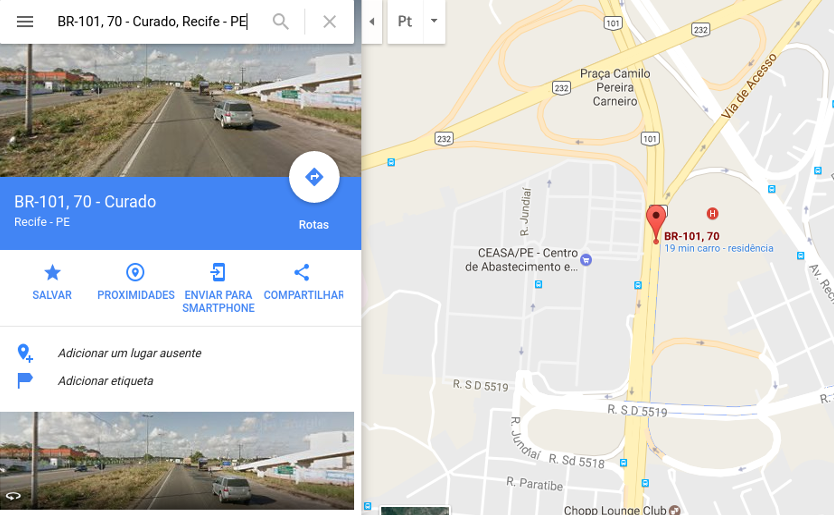
\includegraphics[width=150mm, height=95mm]{Figuras/Resultados/Km70BR101}\\
	\tiny Fonte: Google Maps
\end{figure}

\vspace{7mm}

Em seguida a Matriz de Mortos e a Árvore de Decisão correspondente a esse trecho. Chamamos a atenção para o km 68 desta rodovia o número de óbitos somente neste local é o dobro dos outros. Provavelmente o local mais perigoso para se atravessar em todo Estado de Pernambuco.

\begin{figure}[htbp!]
	\centering
	\caption{Matriz de Mortos: Km 56 -- 78, BR 101 (Sul) Pernambuco}
	\label{fig:MatrizMortos2d-101}
	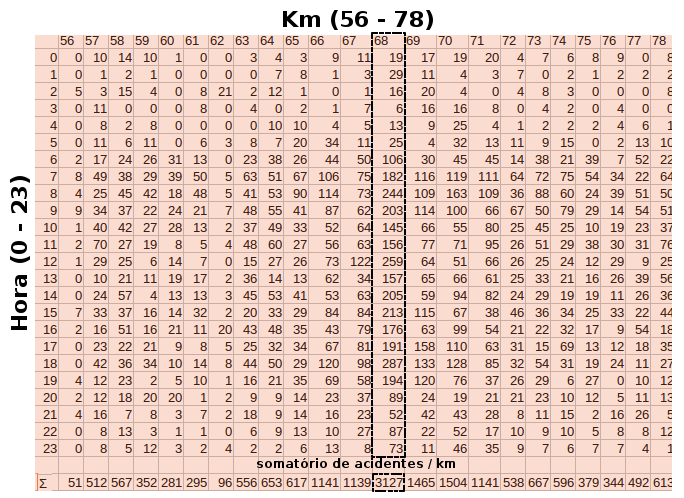
\includegraphics[width=120mm, height=90mm]{Figuras/Resultados/MM2d101}\\
	\tiny Fonte: o Autor
\end{figure}

\pagebreak


%% BR 104
\begin{figure}[htbp!]
	\centering
	\caption{Km 64 e 67, BR 104 Pernambuco}
	\label{fig:Km70BR101}
	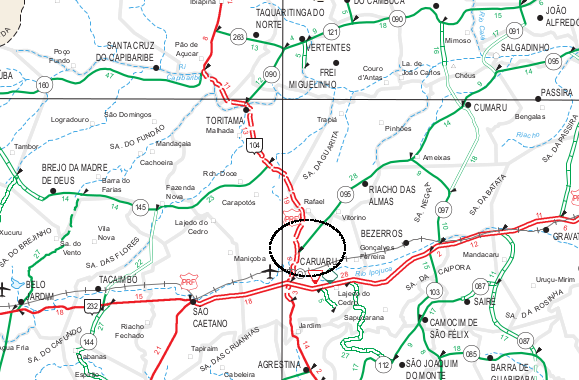
\includegraphics[width=150mm, height=95mm]{Figuras/Resultados/CaruaruRegiao}\\
	\tiny Fonte: Google Maps
\end{figure}

\vspace{7mm}

Em seguida a Matriz de Mortos correspondente a esse trecho. Chamamos a atenção para o km 64 e km 67 desta rodovia o número de óbitos nestes locais é quase o dobro dos outros. Provavelmente este é o local mais perigoso desta rodovia.

\begin{figure}[htbp!]
	\centering
	\caption{Matriz de Mortos: Km 56 -- 78, BR 101 (Sul) Pernambuco}
	\label{fig:MatrizMortos2d-101}
	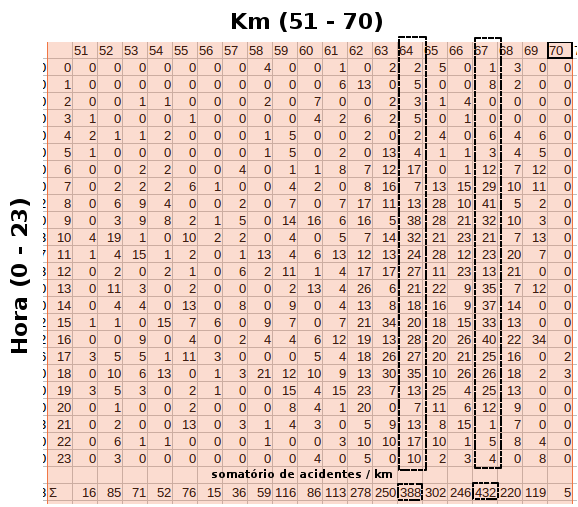
\includegraphics[width=120mm, height=90mm]{Figuras/Resultados/MM2d104}\\
	\tiny Fonte: o Autor
\end{figure}

\pagebreak


Para a região no entorno da BR 116, os acidentes com
mortes [Gravidade = S] ocorrem frequentemente às quinta-feira, envolvendo todos os tipos de veículos.
Os valores das regras encontradas pelo algoritmo para a
variável “Causa do Acidente” foram:
[Ingestão de álcool], [Tipo de auto: não identificado], [Período:
Manhã] o tipo de acidente => colisão traseira.
[Ingestão de álcool], [Tipo de auto: automóvel], [Traçado da
via: Reta], [Condição da pista: molhada], [Dia da semana]:
[Segunda-feira] => colisão frontal
[Terça-feira] => colisão transversal
[Quarta-feira] => colisão transversal
[Quinta-feira] => saída de pista
[Sexta-feira] => colisão traseira
[Sábado]: [BR = 232] => colisão traseira
	[BR > 232] => colisão frontal


\begin{figure}[htbp!]
	\centering
	\caption{Matriz de Gravidade 3D: Br 116 predição para quinta-feira}
	\label{fig:MatrizMortos2d-101}
	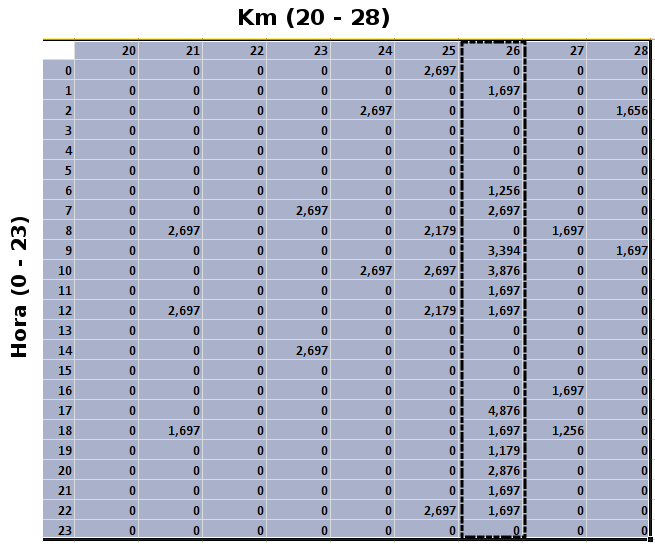
\includegraphics[width=120mm, height=100mm]{Figuras/Resultados/MGrav3D116}\\
	\tiny Fonte: o Autor
\end{figure}


\pagebreak

\subsection{Resultado dos outros classificadores utlizados nesta pesquisa}

Os dados gerados pelos outros classificadores -- Naïve Bayes e Redes Neurais -- permitiram confirmar que os resultados encontrados pelas Árvores de Decisão são os mais adequados para o modelo proposto.

A seguir exemplificamos alguns dos resultados desses classificadores:


\begin{figure}
	\centering
	\caption{Resultado da classificação feita pelo Naïve Bayes -- acurácia}
	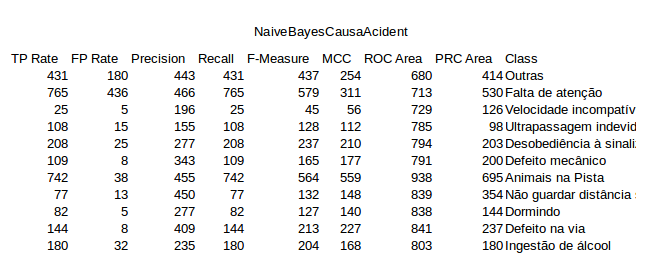
\includegraphics[width=90mm, height=70mm]{Figuras/Resultados/NaiveBayesCausaAcident}\\
	\tiny Fonte: O Autor
	\label{fig:NaiveBayesCausaAcident}
\end{figure}


\begin{figure}
	\centering
	\caption{Resultado da classificação feita pela Rede Neural -- acurácia}
	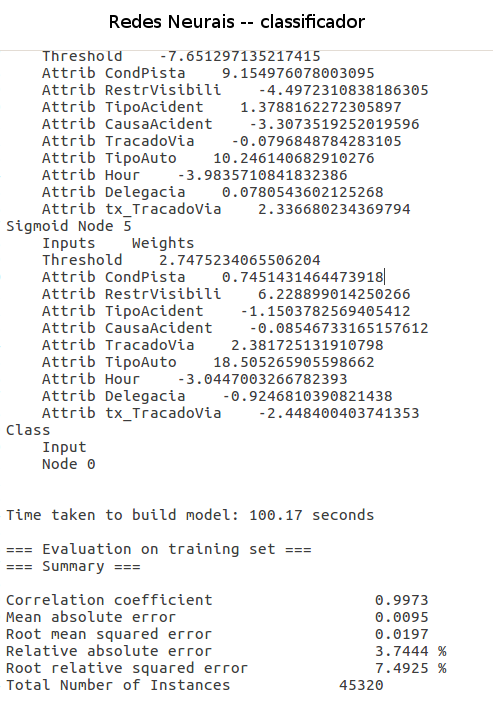
\includegraphics[width=90mm, height=115mm]{Figuras/Resultados/RNN}\\
	\tiny Fonte: O Autor
	\label{fig:RNN}
\end{figure}


\pagebreak

\section{Acoplamento com a estrutura dinâmica}

As predições feitas na primeira fase têm como ``output'' georreferenciamento que localiza um ponto no mapa a partir do quilômetro (Km). O georreferenciamento mais preciso seria a latitude e longitude. Todavia, esses dados apresentaram grave inconsistência na base de dados da PFR/PE, tendo sido descartados. Sentimos necessidade de informações sobre a teoria do fluxo de tráfego, que consiste de leis matemáticas, físicas aplicadas ao tráfego de automóvel, tais como o fluxo (veículos/hora), a velocidade (km/hora) e a densidade de tráfego (veículos/km).

A estrutura dinâmica é composta por duas API's, uma disponibilizada pelo Google, através do Google Maps, que está atualmente na versão V3, e a
outra por uma API do Twitter. A API do Google Maps proporciona uma ``leitura'' atualizada e precisa, de forma que os dados do Km da rodovia podem ser localizados no mapa.

A API do Twitter, por sua vez, possibilita atualizar o utilizador com informações recentes. Contudo, o objetivo desta API é fazer 
um Arco Cibernético das informações, retroalimentando, com dados recentes, um banco de dados de redes sociais. Isso permite um visualização 
instantânea do ambiente como um todo.


\subsection{Mineração em texto no Twitter}

A mineração de dados textuais na rede social Twitter demonstrou ser uma ferramenta promissora, uma vez que oferece uma ampla gama de informações, atualizadas em tempo real. Entretanto, para o caso de pesquisas dessa natureza, o monitoramento precisa ser constante, tendo em vista que novas informações são produzidas a todo momento; e outros canais precisam ser monitorados, a fim de ampliar o universo de dados disponíveis, para produzir o efeito esperado no modelo.

Para localizar novos canais de informação, foram construídos subgrafos contemplando, além dos tweets da PFR, retweets dos seguidores desse canal. Esperava-se, com isso, encontrar novos Hubs na rede. No entanto, a busca em subgrafos é uma tecnologia que precisa ser investigada mais a fundo, dada a sua complexidade.

Conceitos como betwenneess, centralidade, peso das arestas, precisam ser adequadamente compreendidos pelo pesquisador, para que a tecnologia seja explorada em todo seu potencial. Isso implica no estudo de novos algoritmos, próprios para mineração em grafos de redes sociais, o que, em princípio, fugia do escopo dessa pesquisa.

Ainda que consideremos que a ferramenta não tenha sido adequadamente explorada, por todas as questões propostas acima, a mineração de dados textuais do twitter permitiu inferir que o utilizador dessa rede social faz referência ao que acontece nas rodovias, com especial atenção para fatos que possam ter implicação em seu cotidiano, tanto imediatamente (por exemplo, congestionamento numa via que ele utiliza para ir ao trabalho), quanto num universo temporal mais distante (por exemplo, condição da rodovia que dá acesso à cidade em que ele vai passar um feriado). Esse último aspecto é aquele que interessa particularmente ao modelo proposto nessa pesquisa.

Os dados a seguir mostram a busca dos termos frequentes encontrado no documento textual, extraído a partir de 3.200 tweets. O primeiro gráfico apresenta unigramas -- termos frequentes que contém uma palavra -- e bigramas, termos com duas palavras. Foram encontradas palavras como: fiscalização, colisão, vítima fatal, acidentes, detre outros. 

\pagebreak

\begin{figure}
\centering
\caption{Gráfico de frequência de palavras -- unigramas}
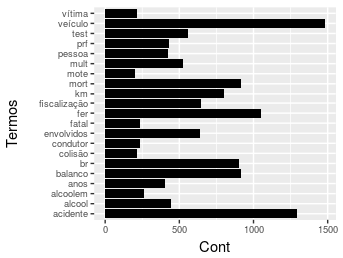
\includegraphics[width=0.7\linewidth]{Figuras/Twitter/freqPalavr}
\label{fig:freqPalavras}
\end{figure}

\quad

A nuvem de palavras é um gráfico de frequência de palavras em que os termos mais frequentes aparecem em destaque -- com letras em tamanho maior -- seguidos pelos próximos termos mais frequentes -- em tamanho um pouco menor -- e assim sucessivamente, chegando a contemplar dezenas ou até centenas de palavras, a depender da escolha do pesquisador. No caso da nuvem de palavras a seguir, aparecem cerca de 50 termos, e destacam-se como mais frequentes (em virtude do tamanho): veículo, BR, acidente (acid), balanço, dentre outras. 

\begin{figure}
\centering
\caption{Nuvem de palavras da Mineração em textos}
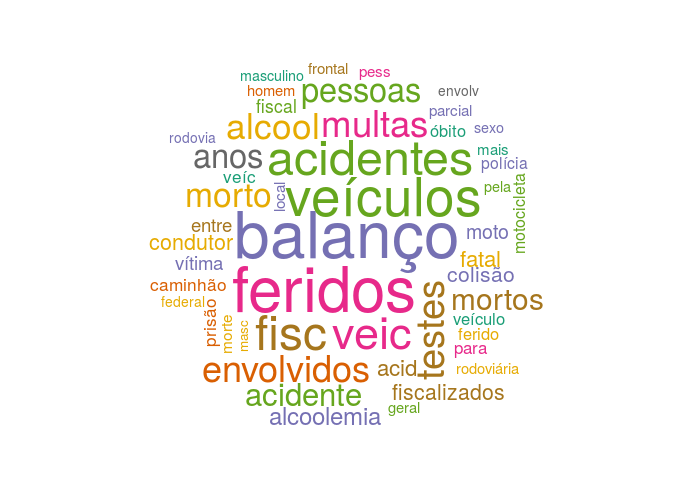
\includegraphics[width=0.5\linewidth]{Figuras/Twitter/nuvem2}
\label{fig:Nuvem1}
\end{figure}


\pagebreak

O dendograma é um gráfico que agrupa palavras de acordo com o assunto. No dendograma a seguir foram identificados seis agrupamentos (clusters), como, por exemplo: ferido, balanço e morto; envolvidos, veículo (veic), fiscalização (fisc), multa, alcoolemia, pessoa, test; PRF; fatal, vítima, envolvido, óbito, prisão, condutor, colisão, moto, ano, h (hora). Os agrupamentos, quando analisados adequadamente, permitem identificar, com um número reduzido de palavras, o acontecimento ao qual está sendo feita referência. Por exemplo, no último agrupamento exemplificado acima é possível deduzir que houve uma colisão envolvendo uma moto, que resultou no óbito de um dos envolvidos e na prisão daquele que foi o responsável pela colisão.   

\begin{figure}
\centering
\caption{Dendograma de Clusterização do resultado da mineração}
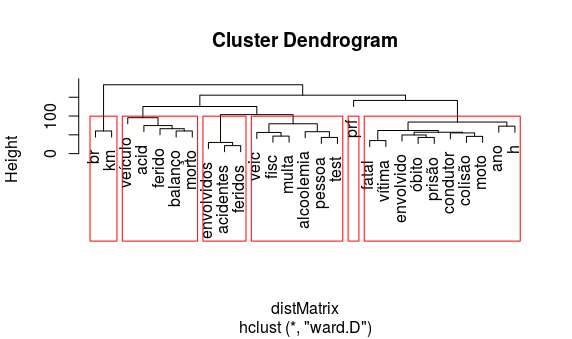
\includegraphics[width=0.7\linewidth]{Figuras/Twitter//Cluster}
\label{fig:Cluster}
\end{figure}

O próximo gráfico ilustra a utilização de outro algoritmo de agrupamento (clusterização), conhecido com K-means. 

\begin{figure}
\centering
\caption{Gráfico da clusterização do resultado da mineração}
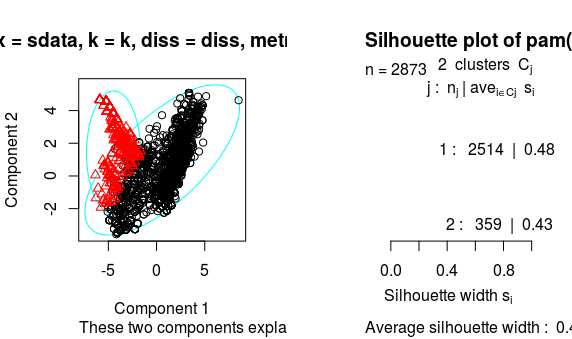
\includegraphics[width=0.7\linewidth]{Figuras/Twitter/Cluster2}
\label{fig:Cluster2}
\end{figure}

Uma análise mais minuciosa dos gráficos produzidos pela mineração de textos pode trazer contribuições de considerável relevância, que permitem refinar o modelo de predição.

%\section{Casos de teste do modelo preditivo}